%\input{preamble.txt}

%\begin{document}
	\section{Android  -- Testing}
	\begin{itemize}
		\item Model-View-Presenter
		\begin{itemize}
			\vspace{0.2cm}
			\begin{minipage}[b]{0.65\textwidth}
				\item An architectural design pattern that results in code that is easier to test
				\item It consists of three components:
				\begin{enumerate}
					\item Model (Data)
					\item View (UI)
					\item Presenter (Business logic)
				\end{enumerate}
			\end{minipage}
			\begin{minipage}[t]{0.2\textwidth}
				\vspace{-3.5cm}
%				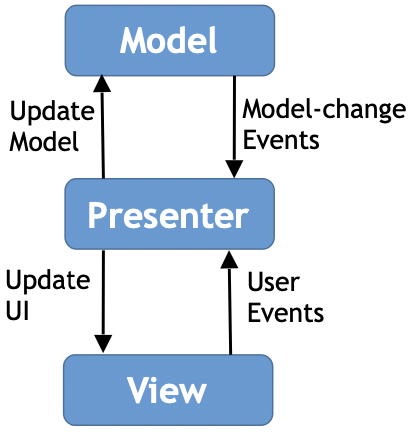
\includegraphics[scale=0.6]{MVP.png}
				\scalebox{0.8}{
					\begin{tikzpicture}
						\node[type, rounded corners, fill=MVPBlue, text=white] (Presenter) {{\Large Presenter}};
						\node[type, rounded corners, fill=MVPBlue, text=white] (Model) [above=of Presenter] {{\Large Model}};
						\node[type, rounded corners, fill=MVPBlue, text=white] (View) [below=of Presenter] {{\Large View}};

						\draw[-Latex, thick] ([xshift=10pt]Presenter.north west) -- ([xshift=10pt]Model.south west) node[left, midway, align=left] {Update \\ Model};
						\draw[-Latex, thick] ([xshift=10pt]Presenter.south west) -- ([xshift=10pt]View.north west) node[left, midway, align=left] {Update \\ UI};

						\draw[-Latex, thick]  ([xshift=-10pt]View.north east) -- ([xshift=-10pt]Presenter.south east) node[right, midway, align=left] {User \\ Events};
						\draw[-Latex, thick]  ([xshift=-10pt]Model.south east) -- ([xshift=-10pt]Presenter.north east) node[right, midway, align=left] {Model-change \\ Events};
					\end{tikzpicture}
				}
			\end{minipage}
		\end{itemize}

		\item Local and Instrumented Tests
		\begin{itemize}
			\vspace{0.2cm}
			\begin{minipage}[b]{0.5\textwidth}
				\item Local unit tests
				\begin{itemize}
					\item Run on the machine’s local JVM
					\item Do not depend on the Android framework
				\end{itemize}
				\item Instrumented tests
				\begin{itemize}
					\item Run on an actual device or an emulator
					\item Usually used for integration and UI tests
				\end{itemize}
			\end{minipage}
			\begin{minipage}[t]{0.4\textwidth}
%				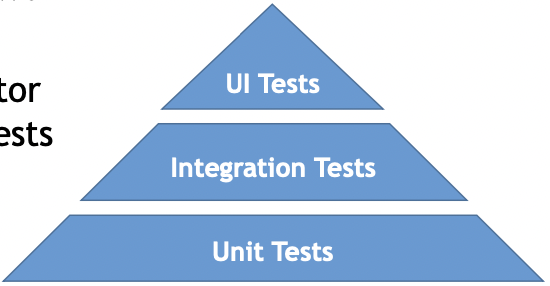
\includegraphics[scale=0.7]{LITests.png}
				\scalebox{0.7}{
					\begin{tikzpicture}
						%				\node[draw,	align=center, regular polygon,	regular polygon sides=3] {UI Tests};
						\coordinate (A) at (0,1.3) {};
						%				\node at (A) [above=1mm of A] {A};
						\coordinate (B) at (1.9,0) {};
						%				\node at (B) [above=1mm of B] {B};
						\coordinate (C) at (-1.9,0) {};
						%				\node at (C) [above=1mm of C] {C};
						\draw[white, fill=MVPBlue] (C)--node [above, midway] {{\LARGE \textcolor{white}{UI Tests}}} (B)--(A)--cycle;

						\coordinate (D) at ([yshift=0pt]C) {}; %%%%%%%%%%%%%%%%%yshift was -10pt
						%				\node at (D) [above=1mm of D] {D};
						\coordinate (E) at ([yshift=0pt]B) {};
						%				\node at (E) [above=1mm of E] {E};
						\coordinate (F) at ([yshift=-1.3cm, xshift=-1.8cm]D) {};
						%				\node at (F) [above=1mm of F] {F};
						\coordinate (G) at ([yshift=-1.3cm, xshift=1.8cm]E) {};
						%				\node at (G) [above=1mm of G] {G};
						\draw[white, fill=MVPBlue] (F) -- (D) -- (E) -- (G) --node [above, midway] {{\huge \textcolor{white}{Integration Tests}}} cycle;

						\coordinate (H) at ([yshift=0pt]F) {};
						%				\node at (H) [above=1mm of H] {H};
						\coordinate (I) at ([yshift=0pt]G) {};
						%				\node at (I) [above=1mm of I] {I};
						\coordinate (J) at ([yshift=-1.3cm, xshift=-1.8cm]H) {};
						%				\node at (J) [above=1mm of J] {J};
						\coordinate (K) at ([yshift=-1.3cm, xshift=1.8cm]I) {};
						%				\node at (K) [above=1mm of K] {K};
						\draw[white, fill=MVPBlue] (J) -- node [above, midway] {{\huge \textcolor{white}{Unit Tests}}} (K) -- (I) -- (H) -- cycle;
					\end{tikzpicture}
				}
			\end{minipage}
		\end{itemize}

		\item Commonly used tools
		\begin{itemize}
			\item JUnit
			\begin{itemize}
				\item Writing unit tests
			\end{itemize}
			\item Mockito
			\begin{itemize}
				\item Creating dummy (mock) objects to facilitate testing a component in
				isolation
			\end{itemize}
			\item Roboelectric
			\begin{itemize}
				\item Running tests that involve the Android framework without an emulator or a device
			\end{itemize}
			\item Espresso
			\begin{itemize}
				\item Writing UI tests
			\end{itemize}
		\end{itemize}

		\item Mock Objects
		\begin{itemize}
			\item A mock is software component that is used to replace the “real” component during testing
			\item Mock objects could be used to:
			\begin{itemize}
				\item Represent components that have not yet been implemented
				\item Speed up testing
				\item Reduce the cost
				\item Avoid unrecoverable actions
				\item Etc.
			\end{itemize}
		\end{itemize}

		\item Mockito
		\begin{itemize}
			\item A mocking framework for Java
			\item Features include:
			\begin{itemize}
				\item Creating mocks
				\item Stubbing
				\item Verifying behavior
			\end{itemize}
		\end{itemize}
	\end{itemize}

%\end{document}